% conventions:
% crossrefs - typechap:name (type: [s]ection,[e]quation,[d]efinition,[t]heorem(lemma,..))
%                           (chap: [p]hysical background, [m]ath tools, [f]luid, [b]odies, [s]teady)
\documentclass[a4paper]{article}
% ***************************************** PACKAGES
\usepackage{amsmath}
\usepackage{amsfonts}
\usepackage{amssymb}
\usepackage{amsthm}
\usepackage{fancyhdr}
\usepackage{graphicx}
\usepackage{natbib}

% ***************************************** SYMBOLS
\def\abs#1{\lvert#1\rvert}
\def\argdot{{\hspace{0.18em}\cdot\hspace{0.18em}}}
\def\avg#1{\left\{#1\right\}_\omega}
\def\D{{\tn D}}
\def\div{\operatorname{div}}
\def\Eh{\mathcal E_h}       % edges of \Th
\def\Ehcom{\mathcal E_{h,C}}         % edges of \Th on interface with lower dimension
\def\Ehdir{\mathcal E_{h,D}}         % Dirichlet edges of \Th
\def\Ehint{\mathcal E_{h,I}}       % interior edges of \Th
\def\grad{\nabla}
\def\jmp#1{[#1]}
\def\n{\vc n}
\def\vc#1{\mathbf{\boldsymbol{#1}}}     % vector
\def\R{\mathbb R}
\def\sc#1#2{\left(#1,#2\right)}
\def\Th{\mathcal T_h}       % triangulation
\def\th{\vartheta}
\def\tn#1{{\mathbb{#1}}}    % tensor
\def\Tr{\operatorname{Tr}}
\def\where{\,|\,}
%***************************************************************************



\begin{document}


\section{Transport of substances}

Flow123d can simulate transport of substances dissolved in water.
The transport mechanism is governed by the \emph{advection}, and the \emph{hydrodynamic dispersion}.
Moreover the substances can move between ground and fractures.
\begin{figure}[h]
\centering
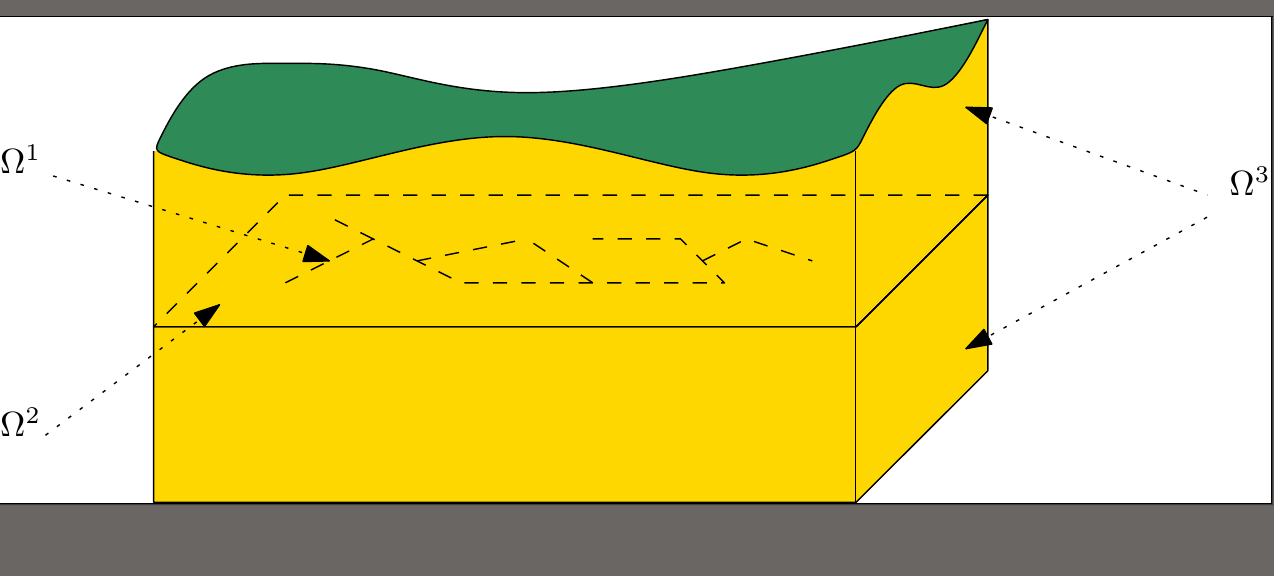
\includegraphics[width=10cm]{ground_fractures}
\end{figure}

\subsection{Physical model}
In the domain $\Omega^d$ of dimension $d\in\{1,2,3\}$, we consider a system of mass balance equations in the following form:
\begin{equation}
    \label{e:ADE}
   \delta^d\partial_t ( \th c^i) + \div ( \vc q^d c^i ) - \div (\th \delta^d \D^i \grad c^i ) = F_S + F_C(c^i) + F_R(c^1,\dots, c^s).%  \quad \text{ in } (0,T)\times\Omega^d.
\end{equation}
The principal unknown is the concentration $c^i$ $[kg\,m^{-3}]$ of a substance $i\in\{1,\dots, s\}$, which means weight of the substance in unit volume of the water.
Other quantities are:
\begin{itemize}
\item $\delta^d$ represents the cross-cut, i.e. $\delta^1$ $[m^2]$ stands for the cross-section, $\delta^2$ $[m]$ for the thickness, and $\delta^3=1$ $[-]$.
\item $\th$ $[-]$ is the porosity, i.e. fraction of space occupied by water and the total volume.
\item $\vc q^d$ $[m^{4-d}\,s^{-1}]$ is the Darcy flux, defined as the product of the \emph{macroscopic} water velocity and the cross-cut.
It is related to the \emph{microscopic} water velocity $\vc v$ $[m\,s^{-1}]$ by the relation $\vc q^d = \th\delta^d\vc v$.
\item The hydrodynamic dispersivity tensor $\D^i$ $[m^2 s^{-1}]$ has the form
\[
  \D^i =D_m^i \tau \tn I + \abs{\vc v}\left(\alpha_T^i \tn I + (\alpha_L^i - \alpha_T^i) \frac{\vc v \times \vc v}{\abs{\vc v}^2}\right),
\]
which represents (isotropic) molecular diffusion, and mechanical dispersion in longitudal and transversal direction to the flow.
Here $D_m^i$ $[m^2\,s^{-1}]$ is the molecular diffusion coefficient of the $i$-th substance (usual magnitude in clear water is $10^{-9}$), $\tau=\th^{1/3}$ is the tortuosity (by \cite{millington_quirk}), $\alpha_L^i$ and $\alpha_T^i$ is the longitudal and the transversal dispersivity $[m]$, respectively.
The value of $D_m^i$ for specific substances can be found in literature (see e.g. \cite{cislerova_vogel}).
For instructions on how to determine $\alpha_L^i$, $\alpha_T^i$ we refer to \cite{marsily,domenico_schwartz}.

\item $F_S$ $[kg\,m^{-d}\,s^{-1}]$ is the density of concentration sources.

\item $F_C(c^i)$ $[kg\, m^{-d}\,s^{-1}]$ is the density of concentration sources due to exchange between regions with different dimensions, see \eqref{e:FC} below.

\item The reaction term $F_R(\dots)$ $[kg\,m^{-d}\,s^{-1}]$ is currently neglected.
\end{itemize}



\paragraph{Initial and boundary conditions.}
At time $t=0$ the concentration is determined by the initial condition
$$ c^i(0,\vc x) = c^i_0(\vc x). $$
The physical boundary $\partial\Omega^d$ is decomposed into two parts:
\begin{align*}
\Gamma_D(t) &= \{\vc x\in \partial\Omega^d\where \vc q(t,\vc x)\cdot\vc n(\vc x)<0\},\\
\Gamma_N(t) &= \{\vc x\in \partial\Omega^d\where \vc q(t,\vc x)\cdot\vc n(\vc x)\ge 0\},
\end{align*}
where $\vc n$ stands for the unit outward normal vector to $\partial\Omega^d$.
On the inflow part $\Gamma_D$, concentrations have to be prescribed (Dirichlet boundary condition):
$$ c^i(t,\vc x) = c^i_D(t,\vc x) \mbox{ on }\Gamma_D(t), $$
while on $\Gamma_N$ we impose homogeneous Neumann boundary condition:
$$ -\th\delta^d\D^i(t,\vc x)\nabla c^i(t,\vc x)\cdot\vc n(\vc x) = 0 \mbox{ on }\Gamma_N(t). $$






\paragraph{Communication between dimensions.}
Transport of substances is considered also on interfaces of physical domains with adjacent dimensions (i.e. 3D-2D and 2D-1D, but not 3D-1D).
Denoting $c_{d+1}$, $c_d$ the concentration of a given substance in $\Omega^{d+1}$ and $\Omega^d$, respectively, the comunication on the interface between $\Omega^{d+1}$ and $\Omega^d$ is described by:
\begin{equation}
  \label{e:inter_dim_flux}
  q^c = \delta^{d+1}\sigma^c (\th^{d+1} c_{d+1} - \th^d c_d) + \begin{cases}q^w c_{d+1} & \mbox{ if }q^w\ge 0,\\q^w c_d & \mbox{ if }q^w<0,\end{cases}
\end{equation}
where
\begin{itemize}
\item $q^c$ $[kg\, m^{-d}\,s^{-1}]$ is the density of concentration flux from $\Omega^{d+1}$ to $\Omega^d$,
\item $\sigma^c$ $[m\,s^{-1}]$ is a transition parameter.
Its nonzero value causes mass exchange between dimensions whenever the concentrations differ.
It is recommended to set either $\sigma^c=0$ (exchange due to transport only) or $\sigma^c \approx\frac{\delta^{d+1}}{\delta^d}|\D|$.
\item $q^w$ $[m^{3-d}\,s^{-1}]$ is the water flux from $\Omega^{d+1}$ to $\Omega^d$.
\end{itemize}
Equation \eqref{e:inter_dim_flux} is incorporated as the total flux boundary condition for the problem on $\Omega^{d+1}$ and a source term in $\Omega^d$:
\begin{align}
-\th\delta^{d+1}\D\nabla c_{d+1}\cdot\vc n + q^w c_{d+1} &= q^c,\\
\label{e:FC}
F_C^d &= q^c.
\end{align}



\section{Numerical solution}

For the numerical approximation of the advection-dispersion equation \eqref{e:ADE} we distinguish whether the dispersion $\D$ is present or not.
Since the true solution has qualitatively different properties, we also choose different numerical methods for each case.

\subsection{Pure advection}

\subsection{Advection with dispersion}

For the general case we use the discontinuous Galerkin space approximation and implicit Euler time discretization.
Let $\tau$, $h$ be the time step and the space discretization parameter, respectively.
We assume that $\Th^d$ is a regular partition of the domain $\Omega^d$ into simplices, $d=1,2,3$.
We define the set $\Eh^d$ of all edges of elements in $\Th$ (triangles for $d=3$, line segments for $d=2$ and points for $d=1$).
Further, $\Ehint^d$ will denote interior edges, $\Ehdir^d(t)$ edges that coincide with $\Gamma_D^d(t)$ and $\Ehcom^d$ stands for edges on interface with $\Omega^{d-1}$.

Let us fix one substance and the space dimension $d$.
At each time instant $t_k=k\tau$ we search for the concentration field $c_d^{h,k}\in V_d^h$, where
$$ V_d^h = \{v:\overline{\Omega^d}\to\R\where v_{|T}\in P_1(T)~\forall T\in\Th^d\} $$
is the space of functions piecewise affine on the elements of $\Th^d$, possibly discontinuous across the element interfaces.
The initial concentration $c^{h,0}_d$ is set to the projection of the initial data $c_0$.
For $k=1,2,\ldots$, the discrete problem reads:
$$ \sc{\th\frac{c_d^{h,k}-c^{h,k-1}_d}\tau}{v}_{\Omega^d} + a^{h,k}_d(c^{h,k}_d,v) = b^{h,k}_d(v) \quad \forall v\in V^h_d. $$
Here $\sc{f}{g}_{\Omega^d}=\int_{\Omega^d} f g$, $c^{h,k-1}_d$ is the solution from the previous time step and the forms $a^{h,k}_d$, $b^{h,k}_d$ are defined as follows:
\begin{multline*}
a^{h,k}_d(u,v) = \sc{\th\D\nabla u}{\nabla v}_{\Omega^d}
+ \sc{(\div\vc q)u}{v}_{\Omega^d}
+ \sc{\vc q\cdot\nabla u}{v}_{\Omega^d}\\
- \sum_{E\in\Ehint^d}\left(\sc{\avg{\th\D\nabla u}\cdot\n}{\jmp{v}}_E + \sc{\avg{\th\D\nabla v}\cdot\n}{\jmp{u}}_E\right)\\
- \sum_{E\in\Ehint^d}\sc{\vc q\cdot\n\avg{v}}{\jmp{u}}_E
+ \sum_{E\in\Ehint^d}\gamma_E\sc{\jmp{u}}{\jmp{v}}_E
+ \sum_{E\in\Ehdir^d(t_k)}\gamma_E\sc{u}{v}_E,
\end{multline*}
% 
\begin{equation*}
b^{h,k}_d(v) = \sum_{E\in\Ehdir^d(t_k)}\gamma_E\sc{c_D}{v}_E.
\end{equation*}
For an interior edge $E$ we denote by $T^-(E)$ and $T^+(E)$ the elements sharing $E$.
By $\n$ we mean the unit normal vector to $E$ pointing from $T^-(E)$ towards $T^+(E)$, the inter-element jump is defined as $\jmp{f}=f_{|T^-(E)}-f_{|T^+(E)}$, and $\avg{f}=\omega f_{|T^-(E)} + (1-\omega) f_{|T^+(E)}$ denotes a weighted average of the quantity $f$.
The weight $\omega$ is chosen in a specific way (see \cite{ern_stephansen_zunino} for details) taking into account possible inhomogeneity of $\D$.
The stabilization parameter $\gamma_E>0$ is user dependent; its value affects the inter-element jumps of the solution.

% \paragraph{Communication between regions of the same dimension.}
In case that lower dimensional domains ($\Omega^1$, $\Omega^2$) have complex topology, e.g. if there are more triangles sharing one line segment, then we consider ideal mixing, i.e. the concentration entering the edge through every inlet element ($\vc q$ points out of this element) is divided among all outlet elements proportionally to their fluxes.

If there are interfaces between adjacent dimensions, then the following terms are added to the bilinear form and the right hand side, respectively:
$$ a^{h,k}_{d,C}(u,v) = \sum_{E\in\Ehcom^d} (\sigma^c+(q^w)^-)\sc{u}{v}_E - \sum_{T\in\Th^d\cap\Ehcom^{d+1}} \frac{\delta_{d+1}}{\delta_d}(\sigma^c+\abs{q^w})\sc{u}{v}_T, $$
$$ b^{h,k}_{d,C}(v) = \sum_{E\in\Ehcom^d} (\sigma^c+(q^w)^-)\sc{c^h_{d-1}}{v}_E - \sum_{T\in\Th^d\cap\Ehcom^{d+1}} \frac{\delta_{d+1}}{\delta_d}(\sigma^c+\abs{q^w})\sc{c^h_{d+1}}{v}_T. $$
Here we obviously set $\Ehcom^4=\Ehcom^1=\emptyset$.

% TODO:
% \begin{itemize}
%   \item Write equations for sorption and integrate them into \eqref{e:ADE}. 
% $R_i(\argdot)$ is a ``retardation function'' its a function which includes various types of equilibrium sorption.
% It is in general dependent as on the substance $i$ as on the material in particular location in space. 
% 
% \end{itemize}
% 
% 
% 
% 
% \begin{enumerate}
%  \item Explicit solution - technicaly this is only slight modification of the already implemented transport model. One has to add appropriate 
%        diffusive flux approximation. Something was done by Sembera nad Jiranek, however there are more possible approximations (further search). Weakness:
%        \begin{itemize}
%         \item too restrictive condition on timestep size for big diffusion on small elements
% 	      \[
% 	         dt \le \min \frac{dx^2}{2D},\qquad dt\le \min \frac{dx}{v}
% 	      \]
% 	\dots so the former condition is more restrictive if $\min dx / D \le 2\min 1/v$ \dots Peclet number can not be used since it 
%         measure only local balnace between diffusion and convection
% 
%         \item persisting problems with CFL condition
%         \item problems with approximation of the diffusive flux with anisothropy raising from the dispersion
%        \end{itemize}
%   \item Implicit solution
%   \begin{enumerate}
%        \item Finite volumes/ Discontinuous Galerkin - search for suitable approximation of the diffusive flux (as above)
%        \item Lumped MH  for diffusion, upwind for convection. Problem with zero or nearly zero $\tn D$. There has to be also implementation without
%              diffusion (no whole MH stuff). Problem that with lumping this leads to edge centered finite volumes.
%   \end{enumerate}   
%   
% \end{enumerate}



\bibliographystyle{abbrvnat}
\bibliography{ref}


\end{document}
